\chapter{Proposed approach}
\label{chapter:proposedApproach}

Describe your approach!

Describe in reasonable detail the algorithm you are using to address this problem. A psuedocode description of the algorithm you are using is frequently useful. Trace through a concrete example, showing how your algorithm processes this example. The example should be complex enough to illustrate all of the important aspects of the problem but simple enough to be easily understood. If possible, an intuitively meaningful example is better than one with meaningless symbols.



Item example: 

\begin{itemize}
	\item content of item1
 	\item content of item2
 	\item content of item3
\end{itemize}



Figure example 

$\ldots$ (see Figure \ref{swarmsize})

\begin{figure}[htbp]
	\centerline{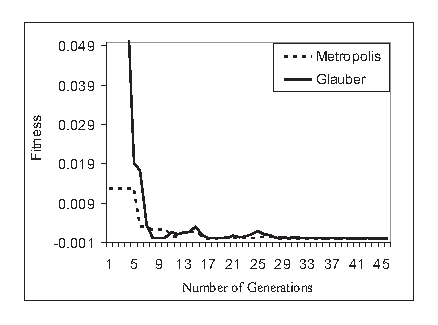
\includegraphics{figures/FitEvol.eps}}  
	\caption{The evolution of the swarm size during the GA generations. This results were obtained for the $f_2$ test function with 5 dimensions.}
	\label{swarmsize}
\end{figure}


Table example: (see Table \ref{tab3PSO})


\begin{table}[htbp]
	\caption{The parameters of the PSO algorithm (the micro level algorithm) used to compute the fitness of a GA chromosome.}
	\label{tab3PSO}
		\begin{center}
			\begin{tabular}{p{220pt}c}

				\textbf{Parameter}& \textbf{Value} \\
				\hline\hline
 				Number of generations& 50 \\
 				Number of function evaluations/generation& 10 \\
 				Number of dimensions of the function to be optimized& 5 \\
 				Learning factor $c_{1}$& 2 \\
 				Learning factor $c_{2}$ & 1.8\\
 				Inertia weight& 0.5 + $\frac{rand()}{2}$\\
		
			\end{tabular}
		\end{center}
\end{table}

Algorithm example 

$\ldots$ (see Algorithm \ref{NGalg}).


\algsetup{indent=1em, linenosize=\footnotesize}

\begin{algorithm}
	\caption{SGA - Spin based Genetic AQlgorithm}
	\label{NGalg}
		\begin{algorithmic}


			\STATE \textbf{BEGIN}
  		\STATE @ Randomly create the initial GA population.
  		\STATE @ Compute the fitness of each individual.
  		\FOR{i=1 TO NoOfGenerations}
  			\FOR{j=1 TO PopulationSize}
  				\STATE p $\leftarrow$ RandomlySelectParticleFromGrid();
  				\STATE n $\leftarrow$ RandomlySelectParticleFromNeighbors(p);
  				\STATE @ Crossover(p, n, off);
  				\STATE @ Compute energy $\Delta H$
  				\IF {$\Delta H$ satisfy the Ising condition}
  					\STATE @ Replace(p,off);
  				\ENDIF
  			\ENDFOR
  		\ENDFOR
  		\STATE \textbf{END}
\end{algorithmic}
\end{algorithm}


